\chapter{Implementation}
\noindent\rule{\linewidth}{2pt}

\section{Introduction}

This chapter presents the implementation details of CropLens AI, covering all four machine learning models, the FastAPI backend, the React frontend, the agricultural knowledge base, the Gemini explanation engine, output interfaces, and the Detailed Disease-Specific Explanation vertical infographic timeline.

\section{Machine Learning Model Training}

\subsection{Leaf Gate Training (\texttt{train\_leaf\_gate.py})}

The Leaf Gate was trained using the PlantVillage dataset (positive class) combined with a collection of non-leaf images (negative class):
\begin{itemize}
    \item Architecture: ImageNet-pretrained MobileNetV2 with binary classifier head.
    \item Optimiser: Adam, learning rate = 0.001.
    \item Loss: Binary Cross-Entropy.
    \item Threshold calibration: \texttt{calibrate\_threshold()} sweeps from 0.1 to 0.9 in steps of 0.01. Final threshold = 0.90, minimising FAR while keeping FRR $\leq$ 2.5\%.
    \item Output: \texttt{leaf\_gate\_mobilenetv2\_best.pth}
\end{itemize}

\subsection{Disease Classifier Training (\texttt{train\_disease.py})}

\begin{itemize}
    \item Dataset: PlantVillage / New Plant Diseases Dataset --- 87,867 images.
    \item Architecture: ImageNet-pretrained MobileNetV2, frozen backbone, retrained head.
    \item Input: 224$\times$224 RGB tensors, ImageNet normalisation.
    \item Optimiser: Adam (lr = 0.001), 5 epochs, Cross-Entropy Loss.
    \item Best validation accuracy: \textbf{97.09\%}, Cross-Entropy Loss: \textbf{0.114}.
    \item Output: \texttt{disease\_mobilenetv2\_best.pth}
\end{itemize}

\subsection{Severity Model Training (\texttt{train\_severity\_conditioned.py})}

\begin{itemize}
    \item Dataset: AI Challenger 2018 --- 37,721 labelled images (26,407 train / 5,667 val / 5,647 held-out test).
    \item Zero-leakage methodology: SHA-256 hash-based deduplication across all splits.
    \item Architecture: \texttt{DiseaseConditioned-}\allowbreak\texttt{MobileNetV2} (MobileNetV2 backbone + 32-dim disease embedding, concatenated 1,312-dim feature, binary classifier head).
    \item 14 supported disease pairs: Corn/Northern Leaf Blight, Corn/Gray Leaf Spot, Corn/Rust, Peach/Bacterial Spot, Pepper/Bacterial Spot, Potato/Early Blight, Potato/Late Blight, Tomato/Bacterial Spot, Tomato/Early Blight, Tomato/Gray Leaf Spot, Tomato/Late Blight, Tomato/Leaf Mold, Tomato/Septoria Leaf Spot, Tomato/Spider Mites.
    \item Held-out Macro-F1: \textbf{95.57\%} (Mild F1: 95.44\%, Severe F1: 95.70\%).
    \item Output: \texttt{severity\_conditioned\_mobilenetv2\_best.pth}
\end{itemize}

\subsection{Yield Regressor Training (\texttt{train\_yield.py})}

\begin{itemize}
    \item Dataset: 2,596 agronomic rows, 5 features: Fertilizer, Temperature, N, P, K.
    \item Algorithm: scikit-learn \texttt{RandomForestRegressor}, 100 trees, \texttt{random\_state=42}.
    \item Split: 80/20 train/test.
    \item Performance: R\textsuperscript{2} = \textbf{0.9908}, MAE = \textbf{0.1229} t/ha, RMSE = \textbf{0.1863} t/ha.
    \item Output: \texttt{yield\_model.pkl} (serialised with joblib).
\end{itemize}

\section{Backend Implementation (FastAPI)}

\subsection{Main Pipeline (\texttt{main.py})}

The \texttt{run\_crop\_health\_pipeline()} async generator in \texttt{main.py} implements the full eight-stage pipeline as a Server-Sent Events stream:
\begin{itemize}
    \item All four models loaded at FastAPI startup via application lifecycle hooks.
    \item \texttt{get\_severity\_routing()} determines severity cases (A/B/C/D) from a JSON mapping file.
    \item Pandas DataFrame constructed from user farm parameters for Random Forest inference.
    \item Pillow used to validate and preprocess uploaded images.
    \item Crop mismatch detection emits a \texttt{crop\_mismatch} SSE event when the predicted crop differs from the user-specified crop.
\end{itemize}

\subsection{Agricultural Knowledge Base (\texttt{knowledge\_base.py})}

A structured Python dictionary covering all 38 disease classifier labels. Each entry contains:
\begin{itemize}
    \item \texttt{causative\_pathogen}: scientific name, taxonomic category, pathogen type.
    \item \texttt{disease\_overview}: comprehensive disease description.
    \item \texttt{favorable\_conditions}: temperature range, humidity/moisture requirements, soil parameters.
    \item \texttt{characteristic\_symptoms}: foliar symptoms, stem and fruit symptoms, progression.
    \item \texttt{transmission\_and\_spread}: primary vectors, survival mechanisms.
    \item \texttt{prevention\_practices}: cultural and agronomic preventive measures.
    \item \texttt{recommended\_management}: cultural controls, cautionary dosage notes.
    \item \texttt{severity\_interpretation}: severity-specific description.
    \item \texttt{professional\_advice\_triggers}: conditions requiring expert consultation.
    \item \texttt{sources}: reference names and URLs from peer-reviewed extension services.
\end{itemize}

\subsection{Gemini Explanation Engine (\texttt{gemini\_service.py})}

The Gemini service:
\begin{itemize}
    \item Reads \texttt{GEMINI\_API\_KEY} and \texttt{GEMINI\_MODEL} from \texttt{ml-service/.env} via \texttt{python-dotenv}.
    \item Calls \texttt{gemini-3.5-flash-lite} via HTTPS POST with a structured JSON prompt.
    \item HTTPX timeout: connect=10s, read=45s, write=10s, pool=5s.
    \item Handles connection errors, read timeouts, HTTP errors, and invalid JSON separately.
    \item Falls back to \texttt{generate\_grounded\_fallback()} on any failure.
    \item API key is never logged or exposed in responses.
\end{itemize}

\section{System User Interfaces}

\subsection{Landing Page}

The landing page provides the entry point to CropLens AI, featuring project statistics and interactive navigation buttons to begin scanning.

\begin{figure}[H]
\centering
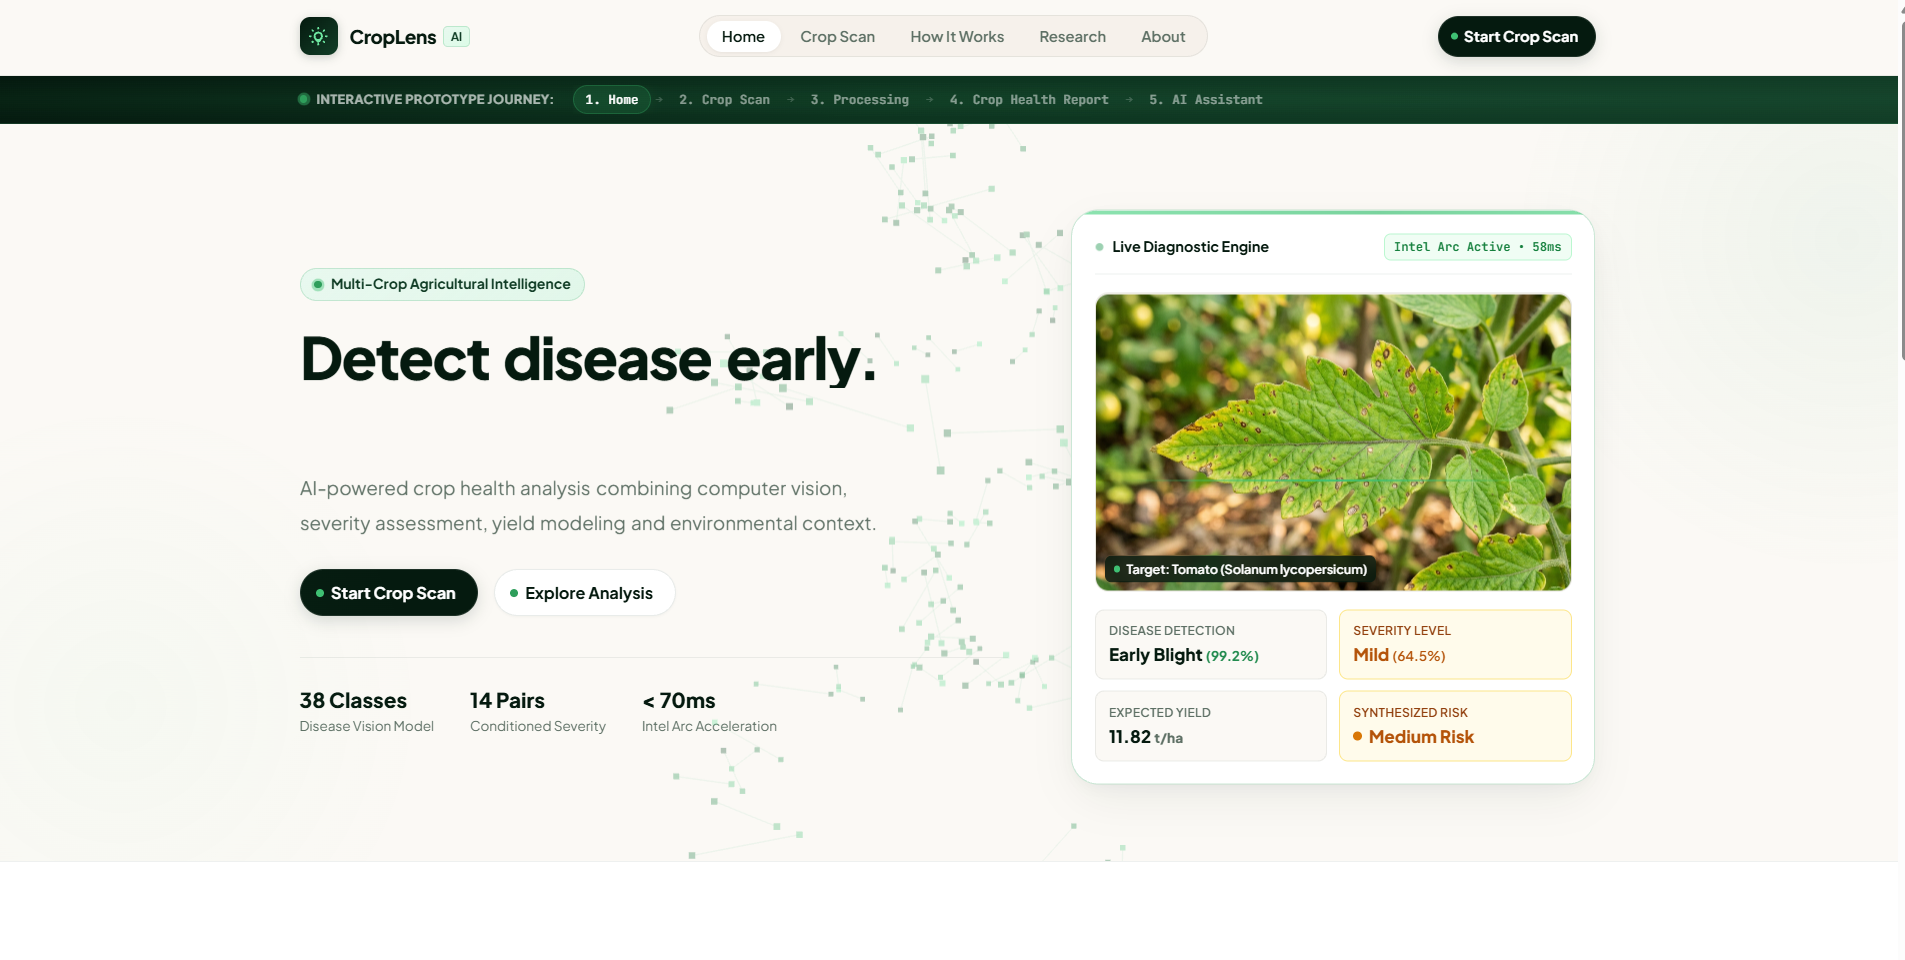
\includegraphics[width=0.92\textwidth]{Figures/output_landing.png}
\caption{CropLens AI Landing Interface}
\label{fig:landing}
\end{figure}

\FloatBarrier

\subsection{Crop Scan Input Form}

The scan interface allows users to upload a leaf photograph and provide soil and climate parameters.

\begin{figure}[H]
\centering
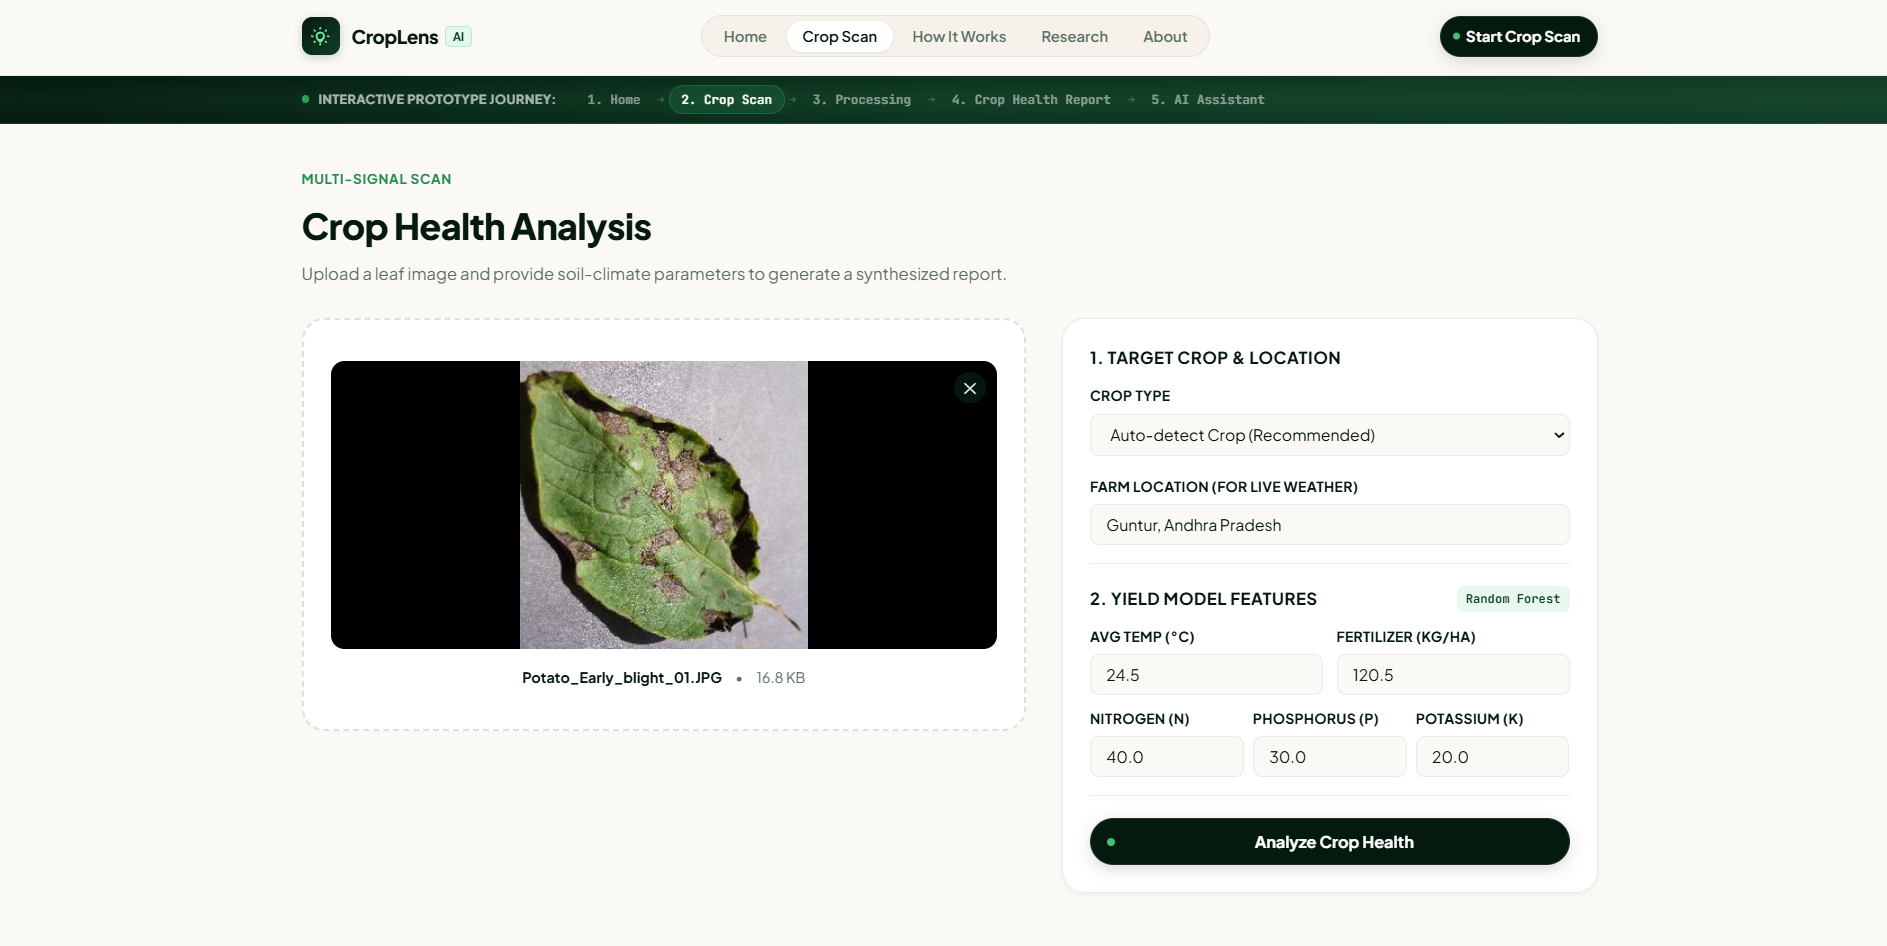
\includegraphics[width=0.92\textwidth]{Figures/output_scan.png}
\caption{Crop Scan Form Interface}
\label{fig:scan}
\end{figure}

\FloatBarrier

\subsection{Real-Time Processing View}

The processing view displays an animated eight-stage pipeline timeline driven by Server-Sent Events emitted by the FastAPI backend.

\begin{figure}[H]
\centering
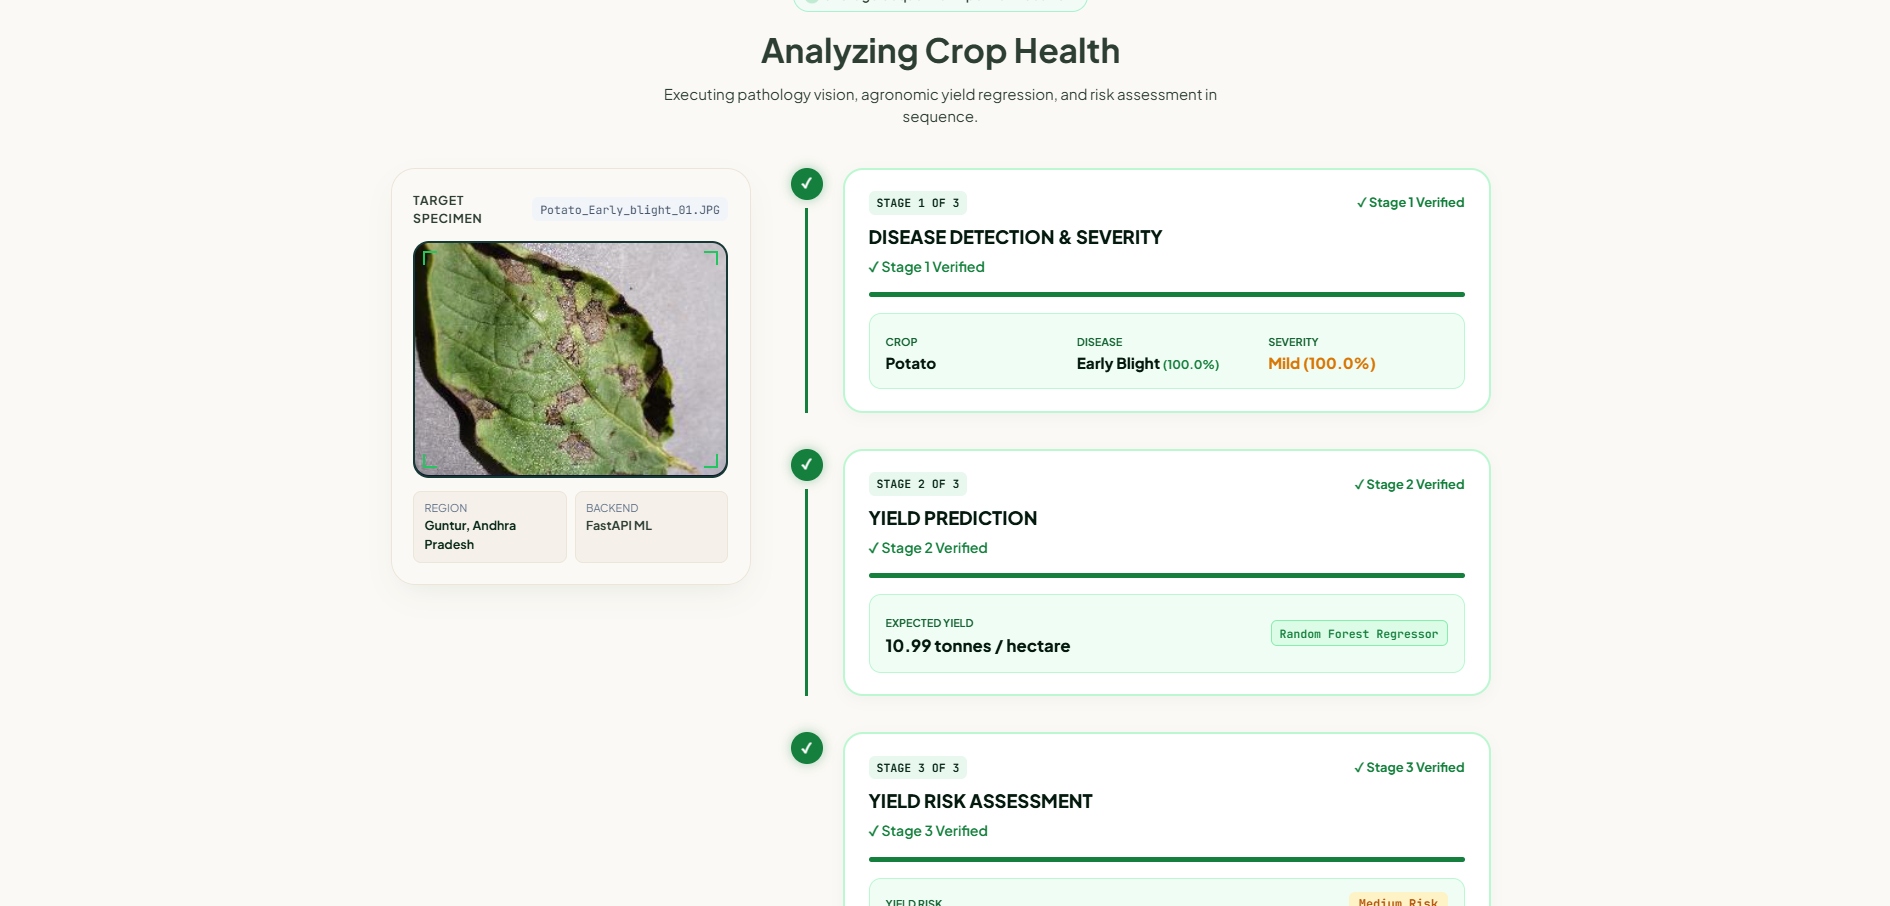
\includegraphics[width=0.92\textwidth]{Figures/output_processing.png}
\caption{Real-Time Pipeline Processing View}
\label{fig:processing}
\end{figure}

\FloatBarrier

\subsection{Crop Health Report}

The crop health report compiles disease diagnosis, severity grade, expected yield, yield risk, and environmental context into a unified dashboard.

\begin{figure}[H]
\centering
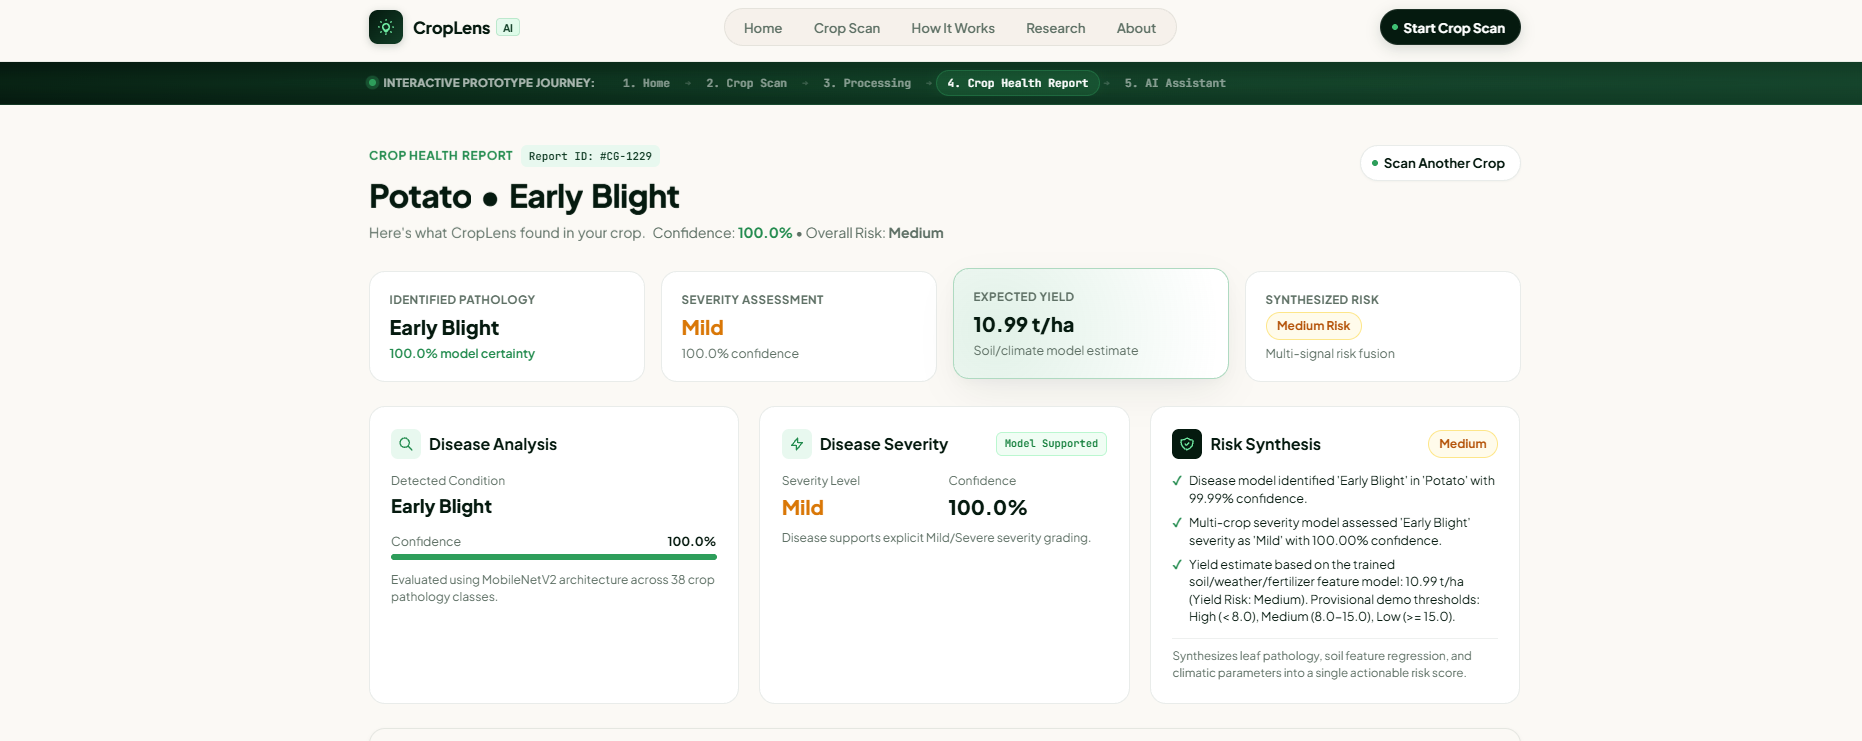
\includegraphics[width=0.92\textwidth]{Figures/output_report.png}
\caption{Crop Health Diagnostic Report Interface}
\label{fig:report}
\end{figure}

\FloatBarrier

\subsection{AI Assistant and Voice Interface}

The AI Assistant provides grounded disease explanations and hands-free voice synthesis for rural accessibility.

\begin{figure}[H]
\centering
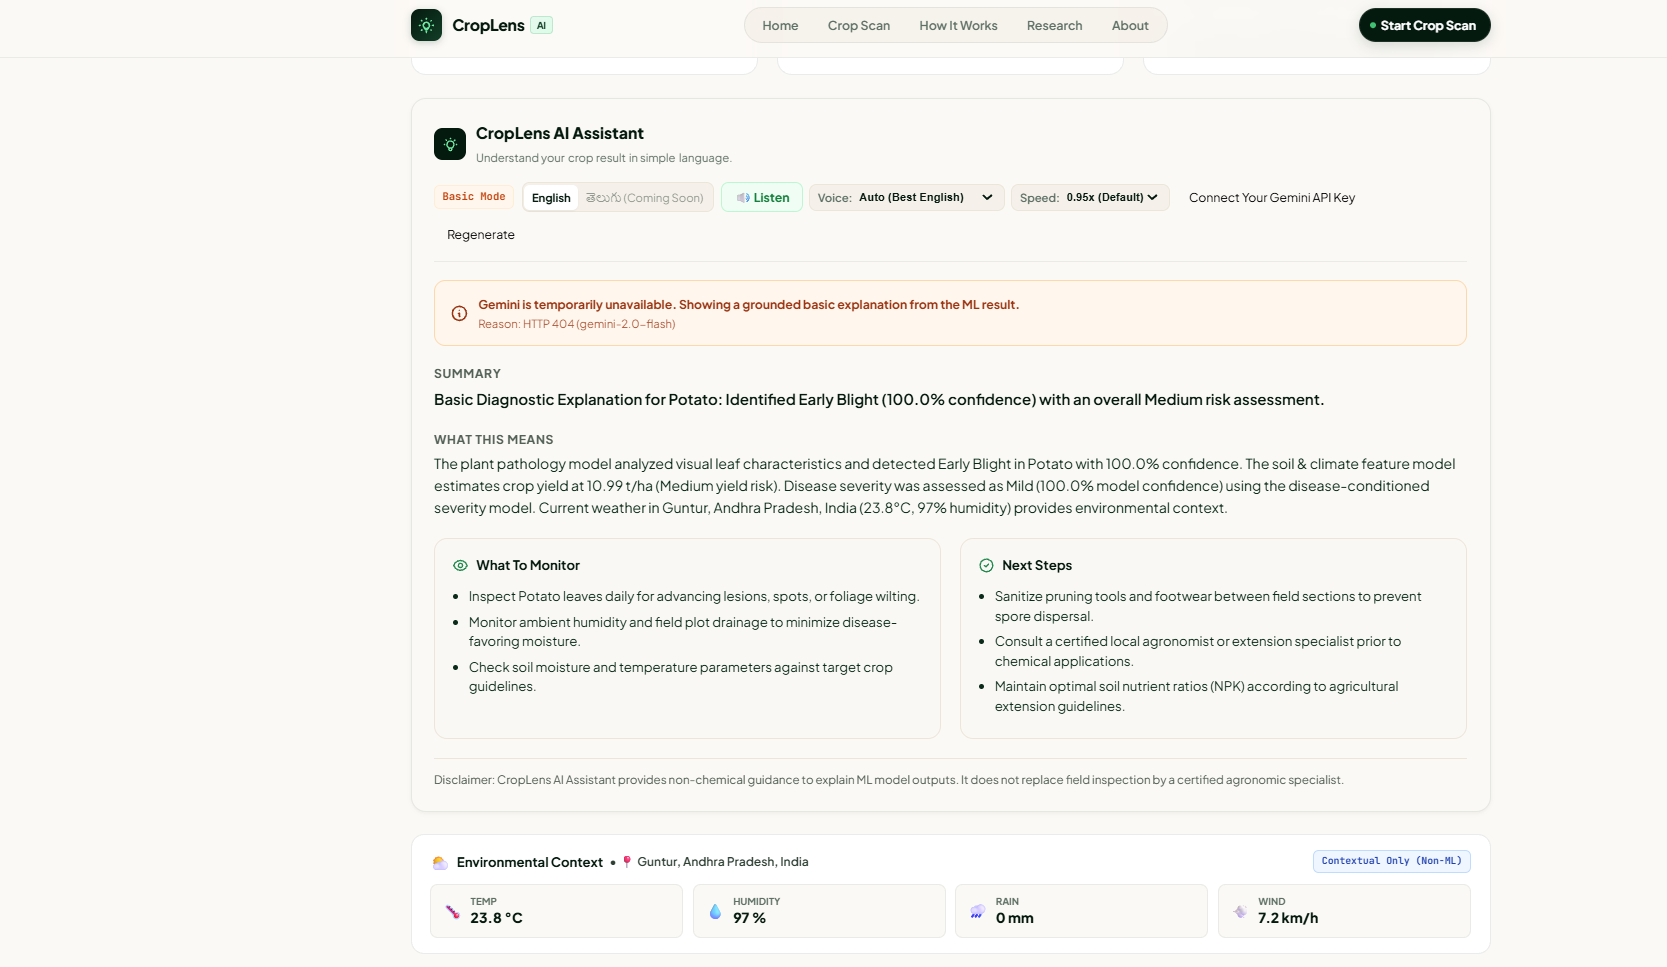
\includegraphics[width=0.92\textwidth]{Figures/output_assistant.png}
\caption{AI Assistant and Grounded Explanation Interface}
\label{fig:assistant}
\end{figure}

\FloatBarrier

\subsection{Detailed Disease-Specific Explanation Timeline}

The Detailed Disease-Specific Explanation section was redesigned as a vertical connected infographic timeline matching professional agricultural publication standards:
\begin{itemize}
    \item \textbf{Continuous vertical spine:} \texttt{.report-timeline-line-track} with an animated botanical-green stroke.
    \item \textbf{Numbered circular badges:} Forest-green badges \texttt{01}--\texttt{08} marking each thematic card.
    \item \textbf{Eight horizontal cards:} Detailed cards with titles, copy, and themed circular icon badges.
    \item \textbf{Tag chips:} Blue chips for weather conditions, purple chips for transmission vectors, and green chips for pathogen taxonomy.
    \item \textbf{Severity Track Gauge:} Dual-gradient horizontal gauge with a dynamically positioned indicator marker.
    \item \textbf{Zero text truncation:} Complete dynamic preservation of all scientific data.
\end{itemize}

Table~\ref{tab:timeline_cards} details the eight timeline cards and their assigned themes.

\begin{table}[H]
\centering
\caption{Detailed Disease-Specific Explanation Timeline Cards}
\label{tab:timeline_cards}
\begin{tabular}{|p{1.4cm}|p{4.2cm}|p{2.6cm}|p{3.6cm}|}
\hline
\textbf{Card \#} & \textbf{Section} & \textbf{Icon} & \textbf{Theme Colour} \\
\hline
01 & Disease Overview & FileText & \#16a34a (Green) \\
02 & Favorable Conditions & Thermometer & \#2563eb (Blue) \\
03 & Characteristic Symptoms & Leaf & \#d97706 (Amber) \\
04 & Transmission \& Spread & Wind & \#7c3aed (Purple) \\
05 & Prevention Practices & Shield & \#0d9488 (Teal) \\
06 & Recommended Management & CheckCircle2 & \#0284c7 (Sky Blue) \\
07 & Severity Interpretation & BarChart2 & \#e11d48 (Coral) \\
08 & Professional Advice Triggers & AlertTriangle & \#9333ea (Magenta) \\
\hline
\end{tabular}
\end{table}

\section{Automated Test Suite}

A pytest test suite validates the complete system with 84 tests across four modules:
\begin{itemize}
    \item \texttt{test\_knowledge\_base.py:} 14 tests verifying coverage of all 38 class labels, healthy class handling, and required field completeness.
    \item \texttt{test\_gemini\_service.py:} 26 tests verifying knowledge base resolution, fallback generation, Gemini mocking, and timeout handling.
    \item \texttt{test\_all\_crop\_coverage.py:} 39 tests verifying end-to-end resolution for every classifier label.
    \item \textbf{Result:} \textbf{84/84 tests passed} in 3.46 seconds with zero regressions.
\end{itemize}

\section{Summary}

This chapter demonstrated the implementation of CropLens AI, including model training, backend endpoints, graphical interfaces, vertical infographic timeline, and the automated test suite confirming end-to-end system reliability.
